%%%%%%%%%%%%%%%%%%%%%%%%%%
%%% Most used packages %%%
%%%%%%%%%%%%%%%%%%%%%%%%%%
\documentclass[a4paper]{memoir}
\usepackage[utf8]{inputenc}
\usepackage[T1]{fontenc}
\usepackage{hyperref}
\usepackage{amsmath}
\usepackage{amssymb}
\usepackage{amsthm}
\usepackage{stmaryrd}
\usepackage{graphicx}
\usepackage{parskip}
\usepackage{pgf}
\usepackage{amsmath}
\usepackage{amssymb}
\usepackage{tikz}
\usepackage{color}
\usetikzlibrary{arrows, automata, positioning}
\usepackage{lstautogobble}
\usepackage[framemethod=tikz]{mdframed}
\usepackage[lofdepth,lotdepth]{subfig}
\usepackage{subcaption}
%%% Used language
\usepackage[english]{babel}

%%% Default margin
\usepackage[left=3cm,right=3cm,top=3cm,bottom=3cm]{geometry}

%%% Default indentation
\setlength{\parindent}{0cm}


%%%%%%%%%%%%%%%%%%
%%% Cover page %%%
%%%%%%%%%%%%%%%%%%
%%% Template link :
%%% http://mirror.jmu.edu/pub/CTAN/info/latex-samples/TitlePages/titlepages.pdf
%%% Many thanks to Peter Wilson for is work.
\newlength{\drop}
\newcommand*{\titleM}{\begingroup % Misericords, T&H p 153
\drop = 0.08\textheight
\centering
\vspace*{\drop}

%%% Document title
{\Huge\bfseries Projet : Un problème de tomographie discrète}\\[\baselineskip]

%%% Document sub-title, can be repeated
{\large\scshape MOGPL : Modélisation et Optimisation par les Graphes et la Programmation Linéaire}\\[\baselineskip]

%%% Center text
\begin{vplace}[0.7]
    \textit{}
\end{vplace}

%%% Authors
{\scshape Realisé par\\ BECIRSPAHIC Lucas\\ et\\ ADOUM Robert}\par

\vspace*{2\drop}
\endgroup}


%%%%%%%%%%%%%%%%%%%
%%% Page number %%%
%%%%%%%%%%%%%%%%%%%
\let\footruleskip\undefined
\usepackage{fancyhdr} 
\fancyhf{}
\cfoot{\thepage}
\pagestyle{fancy}
\renewcommand{\headrulewidth}{0pt}
\renewcommand{\footrulewidth}{0pt}


%%%%%%%%%%%%%%%%%%%%%%%%%%%
%%% Section name format %%%
%%%%%%%%%%%%%%%%%%%%%%%%%%%
\setcounter{secnumdepth}{50}
\setcounter{tocdepth}{50}
\renewcommand{\thesection}{}
\renewcommand{\thesubsection}{}
\renewcommand{\thesubsubsection}{\arabic{section}.\arabic{subsection}.\arabic{subsubsection}}


%%%%%%%%%%%%%%%%%%%%
%%% Environments %%%
%%%%%%%%%%%%%%%%%%%%
%%% Proof
\newenvironment{myproof}[1][\proofname]{\proof[#1]\mbox{}\\*}{\endproof}





\begin{document}
    %%%%%%%%%%%%%%%%%%
    %%% Cover page %%%
    %%%%%%%%%%%%%%%%%%
    \begin{center}
    \titleM 
    \end{center}
    \clearpage
    
    %%%%%%%%%%%%%%%
    %%% Summary %%%
    %%%%%%%%%%%%%%%
    \begin{center}
    \tableofcontents
    \end{center}
    
    %%%%%%%%%%%%%%%%%%
    %%% First page %%%
    %%%%%%%%%%%%%%%%%%
    \newpage
    
    \section{I. Raisonnement par programmation dynamique}
    \subsection{1 - Première étape}
    \textbf{Question 1:}\\\\ Si l’on a calculé tous les $T(j, l)$, pour savoir si il est possible de colorier la ligne $l_{i}$ entière avec la séquence entière  il suffit de de regarder $T(m-1, k)$, si ce dernier vaut vrai alors il est possible de colorier la ligne entière avec la séquence entière. Si il vaut faux alors ce n'est pas possible.\\\\
    \textbf{Question 2:}
    \begin{itemize}
    \item Cas $l = 0$, $j\in{\left\lbrace 0,...,m-1 \right\rbrace }$: Vrai \\
          justification : Si il n'y a pas de bloc à poser, alors un coloriage est toujours possible.
    \item Cas $l \geqslant 1$, $j < s_{l}-1$: Faux \\
          justification : Si le nombre de cases dont on dispose est inférieur à la taille du bloc, on ne peut pas le poser donc faux. 
	\item Cas $l \geqslant 1$, $j = s_{l}-1$:

		\begin{itemize}
			\item Si $l = 1$ alors Vrai 
			\item Si $l \neq 1$ alors Faux
		\end{itemize}
                justification : Si le bloc fait exactement la taille de nos cases, on regarde si il y a un unique bloc à poser. Si ce n'est pas le cas, on renvoi faux.
    \end{itemize}
 	
 	\textbf{Question 3:}\\\\
 	La relation de récurrence permettant de calculer $T(j,l)$ est la suivante:\\\\
 	$T(j, l) = T(j-(s_{l}+1),l-1) \vee T(j-1,l)$\\\\
 	En effet si l'on se trouve à la case j qui est noir, et que l'on veut savoir si il est possible de colorier la sous séquence $(s_{1}, ..., s_{l})$ il faut pouvoir colorier $s_{l}$ case(s) et laisser une case de séparation entre les coloration de $s_{l-1} et s_{l}$, il faut donc regarder si l'on peut colorier la ligne de la case 0 à $j - s_{l} - 1$ avec la sous séquence $(s_{1}, ..., s_{l-1})$. \\
        En revanche si la case j est blanche, il n'est pas possible de placer le bloc par consequent on regarde si il est possible de placer la sequences sur les bloc précédents, ce qui s'exprimer par la formule : $T(j-1,l)$ \\


        \textbf{Question 4:}\\\\
        1) Dans le cas, ou l'on a pas de bloc, il faut vérifier qu'aucune case n'est coloriées.\\
        2.a) Si il n'y a pas la place pour mettre un bloc, c'est toujours faux peu importe la ligne \\
        2.b) Si $j = sl-1$ alors il faut vérifier que l'on peut poser le bloc, c'est à dire il n'y a pas de cases noires sur les cases considérées. \\
        2.c) \begin{itemize}
        \item Si la première case est blanche, on ne peut pas poser le bloc par conséquent on regarde $T(j-1,l)$
        \item Si la case j est noire, on regarde si on peut placer le bloc de manière correcte, c'est à dire pas de blanc sur l'emplacement et un blanc apres et avant pour s'assurer que les blocs son bien séparés.
        \item Si la case n'est pas encore colorié, on traite les deux cas de figures précédent et il suffit qu'un seul soit vrai pour que l'on considère $T(j,l)$ vrai.
          \end{itemize}
        
        

        
        \begin{figure}
          \begin{center}
            \begin{tabular}{|c||c||c|}
              \hline
              instances & nbCases & time \\ 
              \hline
              0 & 20 & 0.00042200088501 \\ 
              \hline
              1 & 25 & 0.000617027282715 \\ 
              \hline
              2 & 400 & 0.117752075195 \\ 
              \hline
              3 & 481 & 0.0961720943451 \\ 
              \hline
              4 & 625 & 0.182909011841 \\ 
              \hline
              5 & 675 & 0.199213027954 \\ 
              \hline
              6 & 900 & 0.51091504097 \\ 
              \hline
              7 & 1054 & 0.300116062164 \\ 
              \hline
              8 & 1400 & 0.43498301506 \\ 
              \hline
              9 & 2500 & 5.42304491997 \\ 
              \hline
              10 & 9801 & 8.71296691895 \\ 
              \hline
            \end{tabular}
            \caption{Tableau représentant les résulats de la programmation dynamique}
          \end{center}
          \end{figure}


\begin{figure}[h]
  \centering
  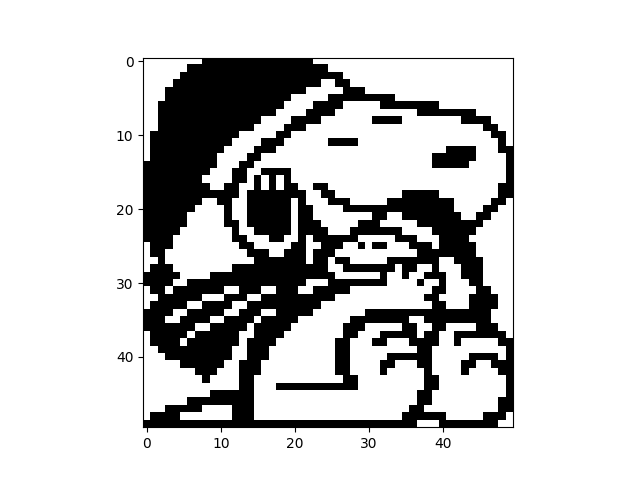
\includegraphics[width=0.75\linewidth]{../images/dynamique_instance9.png}
  \caption{Grille de l'instance numéro 9}
  \label{fig:instance9}
\end{figure}

\textbf{Question 9} En appliquant notre programme sur l'instance 11, on observe qu'en dépit de la petite taille de l'instance notre algorithme ne colorie rien. En effet quand une case peut être colorié à la fois en blanc et en noir notre algorithme ne fais rien. Si la couleur d'une case ne peut être déterminée de manière exacte grace aux contraintes elle ne sera pas colorié. Ce qui explique pourquoi notre algorithme ne colorie pas correctement l'instance 11.
\\
Une solution à ce problème est d'implémenter un algorithme de backtracking qui une fois la coloration effectuée, observe toutes les cases non coloriées et leur affecte 0 et 1 arbirtrairement puis on relance coloration avec la nouvelle grille.
\begin{enumerate}
\item Initialisation : A <- coloration(M) 
\item Tant que la grille n'est pas complete et que le noeud parent n'a pas testé toutes les couleurs:
  \begin{enumerate}
    \item Si coloration(A) != False:\\
      Alors choisir arbritrairement une case incomplete c et lui attribuer une couleur
    \item Si coloration(A) == False:\\
      Alors en retourne à la grille précédente et on attribue l'autre couleur.
    \item  A <- coloration(A)
  \end{enumerate}
\end{enumerate}



 	
 	%\newpage
 	\section{II. La PLNE à la rescousse}
    \subsection{1 - Modélisation}
    \textbf{Question 10:}\\\\ - $x_{ij}$ vaut 1 si la case (i, j)est coloriée en noir et 0 si coloriée en noir.\\\\
    - $y^{t}_{ij}$ vaut 1 si le $t_{ieme}$ bloc de la ligne $l_{i}$ commence à la case (i, j) et 0 sinon.\\\\
    - $z^{t}_{ij}$ vaut 1 si le $t_{ieme}$ bloc de la colonne $c_{j}$ commence à la case (i, j) et 0 sinon.\\\\
    Par conséquent on a : $y^{t}_{ij} = 1 \Rightarrow\sum \limits_{{k=j}}^{j+s_{t}-1} x_{ik} = s_{t}$\\ Et donc $\sum \limits_{{k=j}}^{j+s_{t}-1} x_{ik} = y^{t}_{ij} \times s_{t} $ \\ Par conséquent la condition est: $\sum \limits_{{k=j}}^{j+s_{t}-1} x_{ik} \geq y^{t}_{ij} \times s_{t}  $ \\ Avec le même raisonnement on a pour les colonnes: $\sum \limits_{{k=i}}^{i+s_{t}-1} x_{kj} \geq z^{t}_{ij} \times s_{t} $\\
    \textbf{Question 11:}\\\\
    On cherche à exprimer une contrainte qui empeche de poser un bloc t+1 avant que le bloc t soit posé c'est à dire : 
    $y^{t}_{ij} = 1 \Rightarrow\sum \limits_{{k=0}}^{j+s_{t}} y^{t+1}_{ik} = 0$\\ et $y^{t}_{ij} = 0 \Rightarrow\sum \limits_{{k=j}}^{j+s_{t}} y^{t+1}_{ik} \in \lbrace 0 , 1\rbrace$\\
    Et donc la condition est: $y^{t}_{ij} + \sum \limits_{{k=0}}^{j+s_{t}} y^{t+1}_{ik} \leq 1$\\
    Avec le même raisonnement on a pour les colonnes: $z^{t}_{ij} + \sum \limits_{{k=0}}^{i+s_{t}} z^{t+1}_{kj} \leq 1$\newpage
    \textbf{Question 12:}\\\\
   
  Min z = $\sum \limits_{{i=0, j=0}}^{N, M}x_{i,j}$ \\ 
  $$	
	s.c\left\{
    \begin{array}{ll}
         \sum \limits_{{k=j}}^{j+s_{t}-1} x_{ik} \geq y^{t}_{ij} \times s_{t}$ | $\forall i \in \lbrace 0, 1, 2,...,N-1\rbrace, \forall t \in \lbrace 1, 2,...,k_{i}\rbrace\\\\
         
        \sum \limits_{{k=i}}^{i+s_{t}-1} x_{kj} \geq z^{t}_{ij} \times s_{t} $ | $\forall j \in \lbrace 0, 1, 2,...,M-1\rbrace, \forall t \in \lbrace 1, 2,...,k_{j}\rbrace\\\\
        
        y^{t}_{ij} + \sum \limits_{{k=0}}^{j+s_{t}} y^{t+1}_{ik} \leq 1 $ | $\forall i \in \lbrace 0, 1, 2,...,N-1\rbrace, \forall t \in \lbrace 1, 2,...,k_{i-1}\rbrace\\\\
        
        z^{t}_{ij} + \sum \limits_{{k=0}}^{i+s_{t}} z^{t+1}_{kj} \leq 1$ | $\forall j \in \lbrace 0, 1, 2,...,M-1\rbrace, \forall t \in \lbrace 1, 2,...,k_{j-1}\rbrace\\\\
        
        \sum \limits_{{j=0}}^{M-1} y^{t}_{ij} = 1 $ | $\forall i \in \lbrace 0, 1, 2,...,N-1\rbrace, \forall t \in \lbrace 1, 2,...,k_{i}\rbrace\\\\
        
        \sum \limits_{{i=0}}^{N-1} z^{t}_{ij} = 1 $ | $\forall j \in \lbrace 0, 1, 2,...,M-1\rbrace, \forall t \in \lbrace 1, 2,...,k_{j}\rbrace\\\\
        
      x_{ij} \in \lbrace0,1\rbrace$ | $\forall i \in \lbrace 0, 1, 2,...,N-1\rbrace, \forall j \in \lbrace 0, 1, 2,...,M-1\rbrace\\\\
      
      y^{t}_{ij} \in \lbrace0,1\rbrace $ | $\forall i \in \lbrace 0, 1, 2,...,N-1\rbrace, \forall j \in \lbrace 0, 1, 2,...,M-1\rbrace, \forall t \in \lbrace 1, 2,...,k_{i}\rbrace\\\\
      
      z^{t}_{ij} \in \lbrace0,1\rbrace $ | $\forall i \in \lbrace 0, 1, 2,...,N-1\rbrace, \forall j \in \lbrace 0, 1, 2,...,M-1\rbrace, \forall t \in \lbrace 1, 2,...,k_{j}\rbrace\\\\
    \end{array}\\\\
\right.
$$
\\


\subsection{2 - Implantation et tests}
\textbf{Question 13: }\\\\
(N'oublions pas que j commence à 0 et termine à M-1)\\
- Pour une ligne $l_{i}$ le $l^{ieme}$ bloc ne peut commencer avant la case  $(i, \sum \limits_{{n=1}}^{l-1} (s_{n}+1))$ , ni commencer après la case $(i, M - s_{l} - \sum \limits_{{n = l+1}}^{k_{i}}(s_{n}+1))$ .


\begin{figure}
  \begin{center}
\begin{tabular}{|c||c||c|}
\hline
instances & plne-time & dynamique-time \\ 
\hline
0 & 0.0007050037384033203 & 0.0004220008850097656 \\ 
\hline
1 & 0.0012221336364746094 & 0.0006170272827148438 \\ 
\hline
2 & 2.4385571479797363 & 0.1177520751953125 \\ 
\hline
3 & 0.10664486885070801 & 0.09617209434509277 \\ 
\hline
4 & 9.278510093688965 & 0.1829090118408203 \\ 
\hline
5 & 2.123404026031494 & 0.19921302795410156 \\ 
\hline
6 & 120.54762291908264 & 0.5109150409698486 \\ 
\hline
7 & 0.5048248767852783 & 0.30011606216430664 \\ 
\hline
8 & 1.1952688694000244 & 0.4349830150604248 \\ 
\hline
9 & timeout & 5.423044919967651 \\ 
\hline
10 & timeout & 8.712966918945312 \\ 
\hline
\end{tabular}

\caption{Comparaison des temps pour les 2 methodes}
  \end{center}
  \end{figure}


\begin{figure}[h]
  \centering
  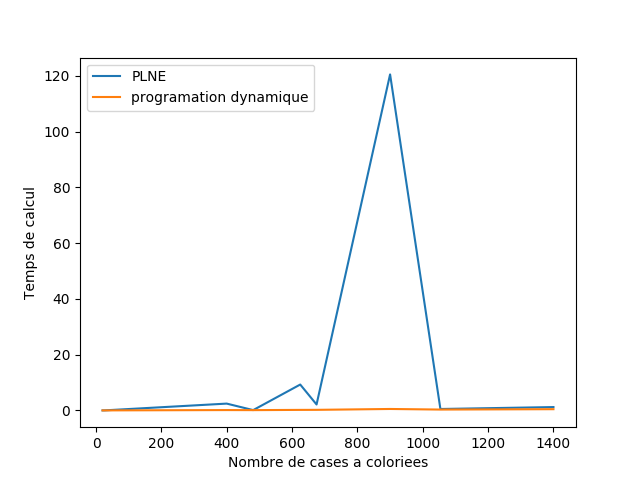
\includegraphics[width=0.75\linewidth]{../graphes/comparaison.png}
  \caption{Comparaison des deux methodes sur les 8 premières instances}
  \label{fig:graphes-comparaison}
\end{figure}

\begin{figure}[h]
  \centering
  \begin{subfigure}
    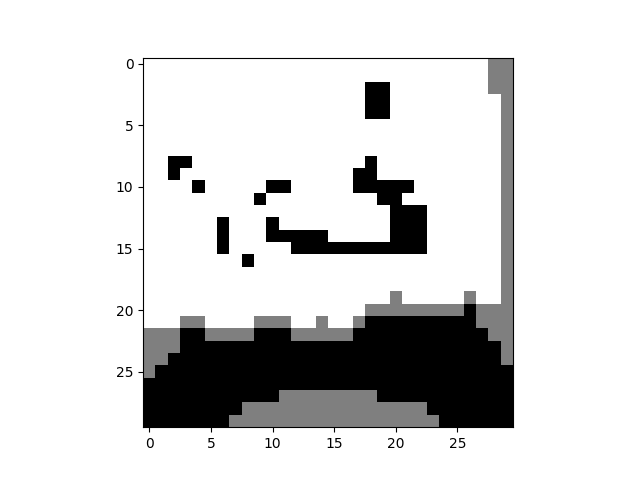
\includegraphics[width=1\linewidth]{../images/dynamique_instance15.png}
    \caption{Images de l'instance 15 avec la programmation dynamique}
    le gris correspond aux cases blanches, le noir aux cases noires et le blanc aux cases non déterminées.
    \label{fig:dynamique15}
  \end{subfigure}
  ~
  \begin{subfigure}
    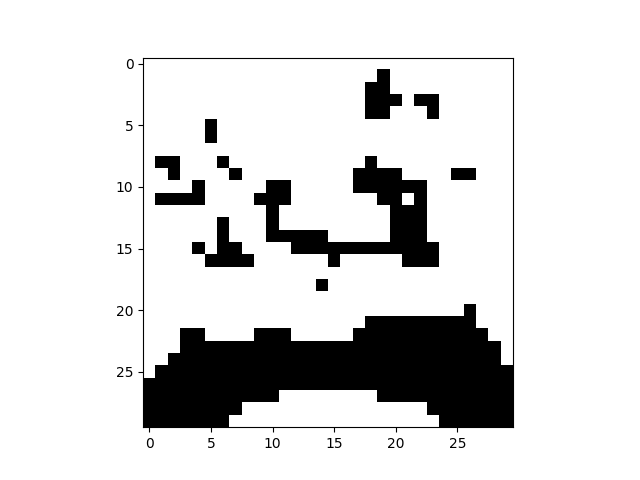
\includegraphics[width=1\linewidth]{../images/plne_instance15.png}
    \caption{Image de l'instance 15 avec la PLNE}
    \label{fig:plne15}
  \end{subfigure}
\end{figure}



\begin{figure}
\begin{tabular}{|c||c||c||c|}
\hline
instances & plne-time & mix-time & nombre de cases \\ 
\hline
11 & 0.0005419254302978516 & 0.0009791851043701172 & 8 \\ 
\hline
12 & 162.9039990901947 & 1.081050157546997 & 924 \\ 
\hline
13 & 2.343104124069214 & 1.3090941905975342 & 2025 \\ 
\hline
14 & 0.7354490756988525 & 0.824674129486084 & 1140 \\ 
\hline
15 & 18.160336017608643 & 7.860313892364502 & 900 \\ 
\hline
16 & timeout & 1650.8602929115295 & 1750 \\ 
\hline
\end{tabular}



\caption{Comparaison des temps entre la plne pure et avec une initialisation avec la programmation dynamique(mix)}
\end{figure}

    
     
\end{document}
